% Apéndice - Modalidad Aero-gestual

\chapter{Modalidad Aero-Gestual} % Chapter title

\label{ch:mod_air} 
Esta modalidad debe ser catalogada inicialmente, dentro del grupo superior de las interfaces gestuales. 
\marginpar{Por interfaces gestuales se hace referencia a aquellas que utilizan movimientos del cuerpo y rostro como señales, que pueden acompañar a la comunicación verbal. En el contexto HCI, el uso de dichas interfaces implica, a través de cámaras o sensores diversos, capturar estos gestos y hacerlos útiles dentro de alguna aplicación.}

En el uso cotidiano que le damos a los gestos, estos suelen complementar la comunicación verbal y son producidos mediante el uso del cuerpo y el rostro. Por esta razón es que esta modalidad tiende a ser usada fácilmente como complemento de otras, \ie~ interfaz de voz.
Una de las ventajas que trae consigo esta interfaz es la universalidad de los gestos en muchos casos, cuando esto ocurre es porque contamos con gestos auto-definidos que rompen las barreras del idioma.

Usualmente encontramos interfaces gestuales en los \emph{pads} de las computadoras portátiles. Un buen ejemplo es el pad de las \emph{ultrabooks}, ya que es común encontrar soporte de numerosos gestos que podemos realizar usando uno o mas dedos.
Al momento de desarrollar cualquier interfaz, si consideramos incluir gestos en la misma, la premisa no debe ser simplemente incluirlos, si no, que tengan un objetivo propio y claro dentro del sistema. 

Uno de los propósitos mas comunes cuando se utilizan interfaces gestuales es el de brindar una forma de trabajo mas ``natural'' al usuario, eliminando cualquier necesidad de hardware extra para interactuar con el sistema, incluso permitiéndole enviar ordenes usando gestos populares, evitando la necesidad de aprender un lenguaje nuevo.

\section{Sentidos Involucrados}
Cuando se habla de gestos, el principal sentido involucrado es el de la visión. Como en muchos otros casos, a través de la vista, recibimos un patrón que cerebro puede detectar muchas veces gracias a nuestro bagaje cultural, aunque en otros casos puede darse que el individuo aprenda un conjunto de gestos nuevos para interactuar con el sistema.

Esta modalidad es de una sola vía, es decir, es un canal de entrada al sistema que no podemos retro-estimular directamente (es posible estimular a otros sentidos como respuesta a un gesto, pero esto es otra cuestión).
Por este motivo y como se menciono anteriormente, esta modalidad suele trabajar en conjunto con otras modalidades en sistemas multimodales, muchas veces funcionando como una herramienta para eliminar ambigüedad introducida por otras interfaces.
 
Los gestos pueden ser clasificados de tres maneras:
\begin{itemize}
\item Semántica; gestos auto-contenidos, comúnmente usados en comunicación no-verbal.
\item Funcional; relacionados al contexto de una aplicación, suelen indicar directivas o comandos, \eg manipulación directa de un elemento.
\item Descriptiva; se concentra en \emph{como} el gesto es realizado.
\end{itemize}

Finalmente, es necesario tener en cuenta la distancia requerida para realizar e interpretar correctamente el gesto, ya que la misma impacta contra el \textit{vocabulario} de gestos a utilizar. Por ejemplo, no es la misma la interacción que podemos tener con una persona frente a frente que si estamos a varios metros de distancia, el conjunto de gestos que usamos cambia. Este es un factor a tener en cuenta cuando se diseña una interfaz gestual.

Particularmente en este trabajo, se hace referencia a interfaces aéreo-gestuales, es decir aquellas que no necesitan de una interfaz externa, como puede ser un dispositivo táctil, para ser usadas; tampoco es necesario que el usuario se acerque a alguna pantalla (aunque esto depende del vocabulario gestual a utilizar). Estas interfaces tienden a usar muy poco o ningún hardware extra, mas allá del dispositivo de escaneo, esto les permite funcionar mas ``naturalmente'', \ie sin necesidad de nada extra en el usuario, posibilitando incluso la captura de gestos conscientes o inconscientes en el usuario.

\section{Interfaces Populares}
Algunas interfaces utilizan técnicas de visión por computadora para detectar los gestos  relevantes del sistema. El trabajo de \citet{wang2009real} es un excelente ejemplo de una técnica efectiva para \emph{trackear}, en este caso, las manos y usarlas como un sistema de gestos funcional, realizando tareas que incluyan manipulación directa con algún elemento de nuestro sistema. 

Otra interfaz que permite capturar información gestual sin necesidad de hardware extra \emph{en el} usuario es el dispositivo \href{https://www.leapmotion.com/}{ Leap Motion}. El mismo utiliza sensores infrarrojos para detectar las manos y triangular posición en tiempo real.
Finalmente, otros dispositivos, populares en sistemas de entretenimiento como son \href{http://www.xbox.com/es-ES/Kinect}{ Kinect, de Microsoft} y \href{http://www.nintendo.com/es_LA/wiiu}{ Wii U de Nintendo}, permiten detectar gestos a nivel cuerpo y a una distancia de un par de metros, generando experiencias de inmersión dentro de los juegos, \emph{trackeando} información gestual del esqueleto humano.

\section{Tecnología Utilizada}
Para este trabajo, se utilizo el dispositivo \textbf{Leap Motion} como herramienta para capturar y acceder a la modalidad aéreo-gestual. Para esto se desarrollo un driver que captura información de uno de los dedos de las manos y la entrega al sistema como si fuera puntero, permitiendo al usuario interactuar de manera funcional con los objetos de la aplicación.

En la figura \ref{fig:apx_airgesture} se puede observar la representación un gesto que puede ser capturado por algún reconocedor, como el mencionado Leap Motion o incluso una cámara web. Este gesto se convierte en una entrada para el sistema que podemos aprovechar, utilizando la plataforma \emph{plusultra}, en el contexto de una aplicación web.

% FIGURA DE MODALIDAD AERO GESTUAL 
\begin{center}
  \begin{figure}[h]
    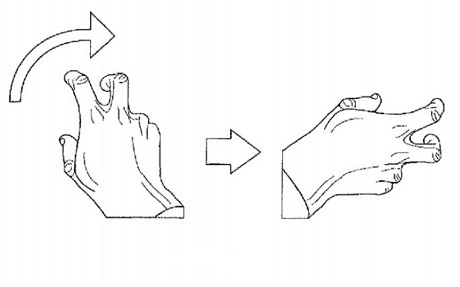
\includegraphics[scale=1,width=\textwidth]{gfx/air-gestures}
    \caption{Representación de un gesto aereo.}
    \label{fig:apx_airgesture}
  \end{figure}
\end{center}
